
Logistics plays an extremely important role in the optimal functioning of humanity as a whole, encompassing the transport of people and goods as well as the provision of services. It is therefore vital that this system operate practically flawlessly and without disruption, but disruptions are unfortunately unavoidable -- the Ever Given container ship grounding incident in the Suez Canal \cite{ref1} is one example. The cause is generally the human factor (inattention, inadequate situational assessment) and/or a technical failure, which can result in an accident.

Preparing vessels and seafarers for navigation is extremely resource-intensive, both financially and in terms of time. The behaviour of the sea is highly unpredictable in open waters, and the risk of drowning is high even under the best preparation; in 2019 drowning deaths ranked third in worldwide cause of death \cite{ref2}, and contributing factors at sea include incompetent preparation (of both the crew and the vessel), overcrowding aboard, excessive trust in the autopilot, and inattention or underestimation of situations.

Long periods at sea are also mentally taxing: there is no direct contact with loved ones, and most of the time is spent in social isolation, except where the crew consists of at least two members. There is also a greater risk of conditions such as hand-arm vibration syndrome (HAVS), cardiovascular disease, pneumonia (in severe cases progressing to lung cancer), general overstrain (caused by muscle tension, excess emotional stress, loneliness that is often suppressed via excessive alcohol consumption and/or smoking, fatigue, and/or insufficient physical activity), and chronic depression \cite{ref3}.

There are several solutions to avoid such problems, of which autonomous control systems using radar and computer vision are currently the most relevant and effective. In the automotive industry, several companies are pursuing full autonomy: Tesla (AutoPilot, FSD) \cite{ref4}, Lucid (DreamDrive) \cite{ref5}, Waymo \cite{ref6}, Nvidia (Nvidia Drive) \cite{ref7}, and Comma.ai (the cheapest semi-autonomous system available) \cite{ref8}.

In the maritime industry, fewer companies have pioneered autonomous systems: Kongsberg \cite{ref9} and Rolls-Royce \cite{ref10}.

An autonomously controlled vessel offers far greater operational efficiency than a crewed one for several reasons: vessel mass is smaller (there is no need for a ventilation system, crew quarters, galley, bunks, sanitation system, or captain's cabin), so less material is required to build it, which in turn improves manoeuvrability. Because the crew is not directly on board, the need for docking is also reduced (only for maintenance/repair, cargo loading, and/or refuelling) and the energy cost of operating the vessel decreases. The vessel can also be sent to operate in harsher conditions without posing a direct risk to human health (and, in the best case, can save time by taking a more direct but more hazardous route).

Tallinn University of Technology and AS Baltic Workboats are partners in a project whose aim is to carry out vessel sea trials autonomously, i.e.\ without human involvement (see Figure 1) \cite{ref11}. There are also plans for further development in the same field, to apply autonomous systems beyond sea trials and give vessels the ability to perform tasks and navigate at sea independently.

\begin{figure}[H]
\centering
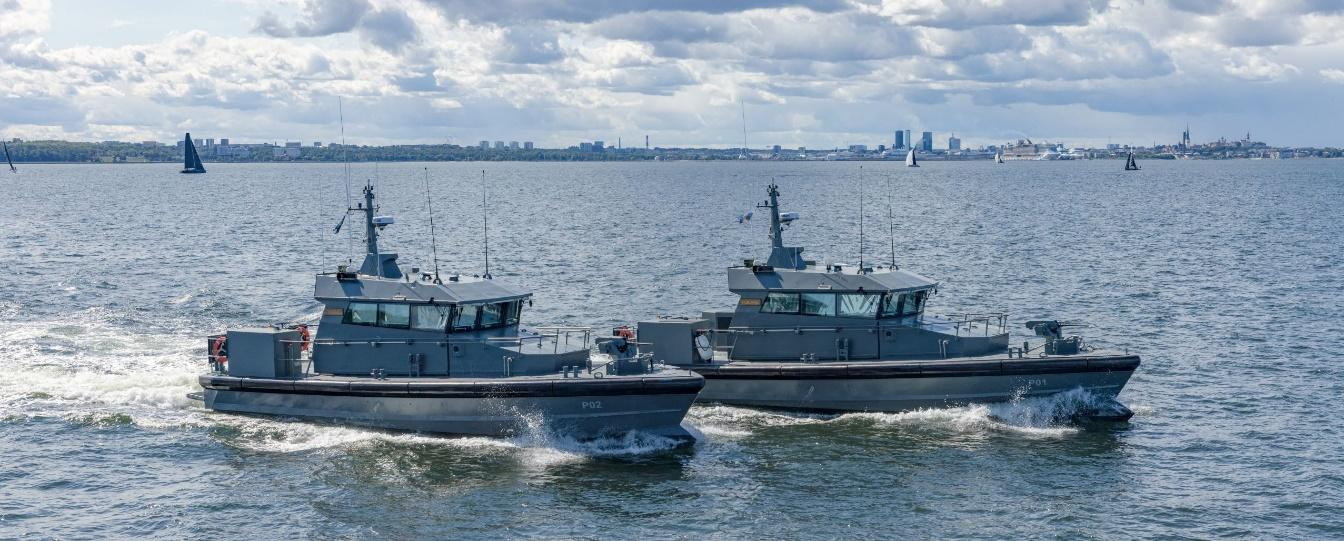
\includegraphics[width=6.10278in,height=2.45694in]{media/image3.jpg}
\caption{Figure 1. Baltic Workboats' Navy 18 WP patrol vessels \cite{ref12}}
\end{figure}

The aim of this bachelor's thesis is to develop a computer vision system that assists with conducting vessel sea trials. This requires selecting suitable hardware, software, and a machine learning model, then creating the computer vision software and optimising the model.

The following questions are addressed in pursuit of this aim:

\begin{itemize}
\item
  Which hardware should be used for the computer vision system?
\item
  Which machine learning model can best detect objects at sea?
\item
  How can objects be detected on an autonomous vessel using computer vision?
\item
  How can the machine learning model be optimised for resource-constrained hardware?
\end{itemize}

The thesis is organised as follows. The Sea trials chapter introduces the methodology of vessel sea trials and the solution for automating them. Chapter 1 discusses computer vision -- its nature and operating principle -- and explains, among the models used in computer vision, the convolutional neural network in particular. Chapter 2 covers the hardware used to build the computer vision system, hardware-level accelerators, and gives a simplified overview of the system. Chapter 3 surveys the different software stacks for building computer vision applications and determines which computer vision model is used in the application. Chapter 4 explains the nature and operating principle of the computer vision application, and describes its development process and optimisation. Chapter 5 carries out experiments with the computer vision models and analyses how much model optimisation affects frame-processing throughput in the application. Chapter 6 summarises the contents and the fulfilment of the thesis's objectives.
